\section{Background}
     
A protocol specification can be broken into four components: message format,
initial configuration, state machine, and system interface. Message formats
define the precise structure of a protocol's messages, their contents, and
invariants. The state machine defines the number of unique protocol states 
which an instance of the protocol may be in, along with guarded transition
functions, transition events, and local state manipulation. The configuration
contains the initial parameters required to instantiate a state machine.
Finally, the system interface defines send/receive message passing, time events,
persistent storage, and a general maintenance. This protocol abstraction is
quite useful in reasoning and testing the protocol design in an independent
manner. This work focuses on a network protocol's message format specification.
Specifically, binary message formats common to network protocols from layers 2-4
will be studied.

Network protocol message formats can be designed and implemented with an
inconsistent structure. 

\begin{figure}[h]
   \begin{center}
   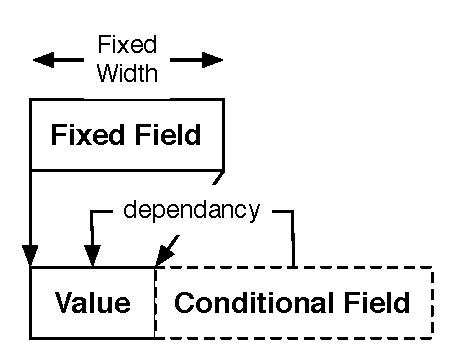
\includegraphics[width=.40\textwidth]{figs/fig1.pdf}
   \caption{Message Format Dependencies}
   \label{figure:fig1}
   \end{center}
\end{figure}

eliminate entire categories of common security
vulnerabilities for network protocol message formats. In particular there are
two common security vulnerabilities that occur in almost all network protocol
implementations: value constraint, and structural constraint violations. A
protocol specification might define a subset of the input range for any
particular value, leaving the remainder unspecified, value constraints are
violated when an implementation blindly handles received values without range
validation allowing for undefined behavior. A structural constraint violation
occurs when a received message describes its structure in a way that violates
the structural rules of the format specification. My first paper focuses on
defining a language for a large subset of IETF binary format based protocols
with the guarantee all well- formed specifications will not allow any type of
value or structural constraint violation. The US- CERT vulnerability database
shows these classes of vulnerabilities exist in current implementations of
simple, old, well understood protocols by extremely knowledgeable organizations~\cite{us_cert}.

\subsection{Network Protocol Problems }

\begin{tabular}{|c|c|c|c|c|}
   \hline
   Age & Protocol & Vendor & Bug Date & US CERT \# \\ \hline
   \hline
   1985 & Bootp & Apple & 2006 & 77628 \\ \hline
   1990 & 802.1q VLAN & Cisco & 2006 & 821420 \\ \hline
   1981 & ICMP & Cisco & 2007 & 341288 \\ \hline
   1985 & NTPD & GNU & 2009 & 853097 \\ \hline
   1998 & OSPFv2 & Quagga & 2012 & 551715 \\ \hline
\end{tabular}

\subsection{Prior Work}

